% twocolumn を使うと2段組になる

%\documentclass[a4j,twocolumn]{jsarticle}        % -> platex
%\documentclass[a4j,twocolumn]{ujarticle}       % -> uplatex
\documentclass[uplatex]{jsarticle}   % -> uplatex + jsarticle

\usepackage{resume} % 他パッケージ,専用コマンド,余白の設定が書かれている

%%%%%%%%%%%%%%%%%%%%%%%%%%%%%%%%%%%%%%%%%%%%%%%%%%%%%%%%%%%%%%%%%%%%%%%%
% ヘッダ: イベント名,日付,所属,タイトル,氏名
%%%%%%%%%%%%%%%%%%%%%%%%%%%%%%%%%%%%%%%%%%%%%%%%%%%%%%%%%%%%%%%%%%%%%%%%

\pagestyle{plain}
\newcommand{\comment}[1]{}
\begin{document}
\twocolumn[
\beginheader{令和5年度 コンピュータサイエンス学部 最終発表}{2023}{2}{1}{井上 研究室}
\title{VRゲーム上で振動刺激のある魔法体験における没入感向上システム}
\author{C0B20032 岡野 真士}
\endheader
]

\vspace{3mm}

 % 本番用ページ番号オフセット
\setcounter{page}{19}
%---------------------------------------------------------------------------
% 本文
%---------------------------------------------------------------------------


\section{はじめに}
Rゲームは360度の視野や立体音響,VRヘッドセットによる身体の動きとの連動させることでプレイヤーの没入感を高めている.
その中で振動刺激は,視覚や聴覚の体験感を補助し,プレイヤーをより仮想世界に没入させる役割を果たしている.
また,VRゲームには魔法を疑似的に体験できるコンテンツが存在する.\cite{maho}

VRゲームでの魔法体験コンテンツの課題として,魔法の形状ごとにどのような振動フィードバックを与えればプレイヤーの魔法体験感を向上させられるのか分かっていない.

本研究では,前述した課題を解決するためにVR上で放った魔法の視覚エフェクトと数種類の振動刺激を組み合わせてユーザーに呈示するシステムを作成する.




%---------------------------------------------------------------------------------------------
\section{関連研究}

\begin{figure}[b]
\centering
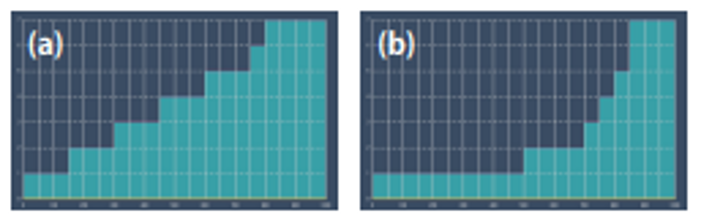
\includegraphics[clip,width=8cm]{fig/vive_patern.png}
\caption{振動パターンの1例}\label{vive}
\end{figure}


スマートフォンにおける多様な振動フィードバックが被験者の印象に与える影響\cite{MetaCookie}の研究を白神らが行った.この研究では振動パターンがユーザーに与える印象に焦点を当て,約250通りの振動パターンからユーザーがどのような印象を持ったのかを調査したものである。

\figref{vive}は振動パターンの一例です。これはジョジョに振動強度が上昇するもので,この振動刺激はユーザーに力強いという印象を与えます。

しかし,実際に存在しているものに関する振動についての調査なので,魔法という非現実的なものに対する振動については明かされていない.


%------------------------------------------------------------------------------------------------
\section{システム概要}
\begin{figure}[b]
\centering
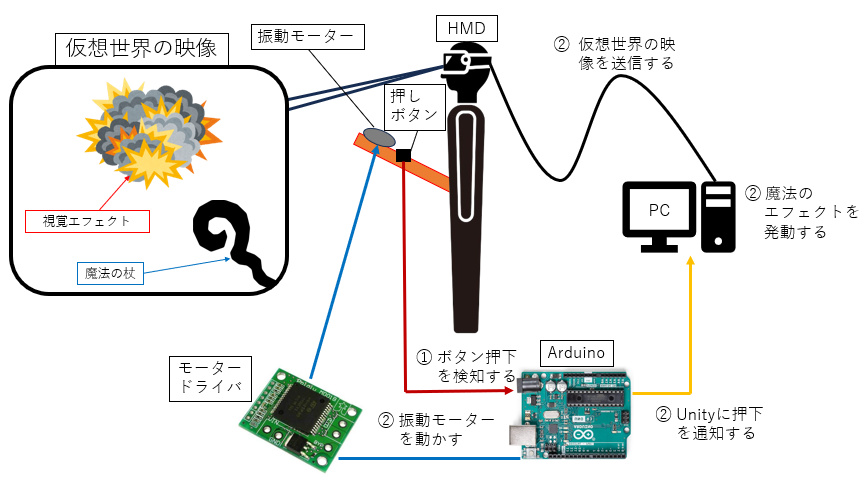
\includegraphics[clip,width=7cm]{fig/systemkousei.png}
\caption{システム概要}\label{system}
\end{figure}

\figref{system}に本システムの構成を示す.
本研究では,被験者が右手にコントローラーを持った状態でHMDを装着する.
被験者がコントローラに装着されている押しボタンを押すことで視覚エフェクトと振動刺激が被験者に提示される.
提示する視覚エフェクトと振動刺激は実験者がPCから決定する.

\section{魔法エフェクトの選定}
実装する視覚エフェクトは,形状が異なりユーザーに与えられる振動刺激が異なると思われる3種類の視覚エフェクトを選定した.

以下に選定した3種類の視覚エフェクトを示す.

incenerationを\figref{fire}に示す.incenerationは火が燃え続けるエフェクトである.
ring-fireを\figref{ringfire}に示す.ring-fireは初めにエネルギーをためるフェーズがあり,その後ためたエネルギーを一気に解放するエフェクトである.
main-beamを\figref{explosion}に示す.main-beamは最初に大きな爆発があり,その後爆発の余韻が残るエフェクトである.

\begin{figure}[h]
\centering
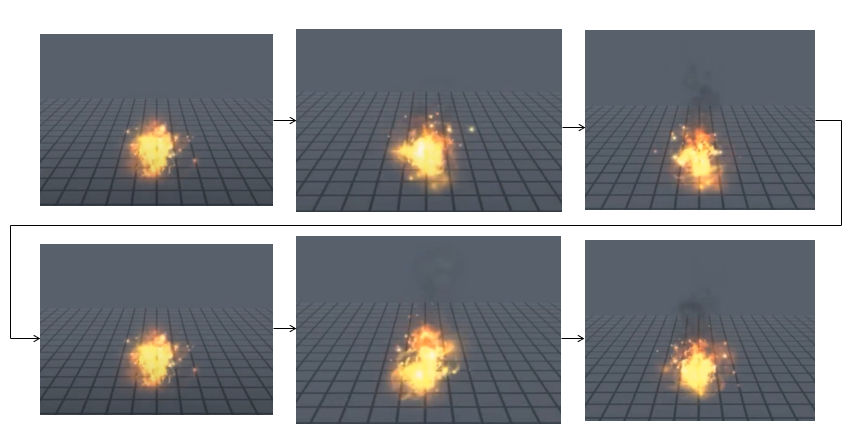
\includegraphics[clip,width=5cm]{fig/fireTime.png}
\caption{inceneration}\label{fire}
\end{figure}

\begin{figure}[h]
\centering
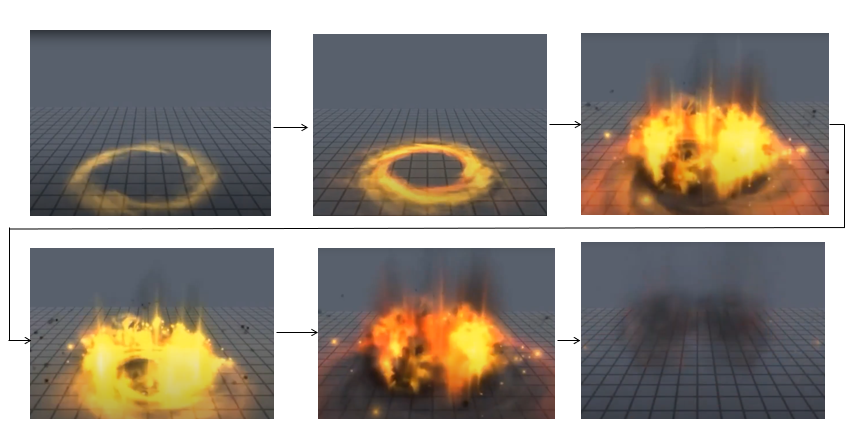
\includegraphics[clip,width=5cm]{fig/ringfireTime.png}
\caption{ring-fire}\label{ringfire}
\end{figure}

\begin{figure}[h]
    \centering
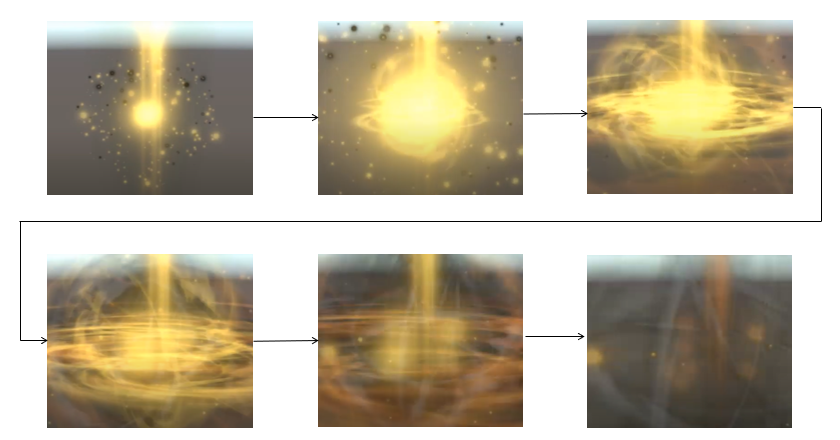
\includegraphics[clip,width=5cm]{fig/mainbeamTime.png}
    \caption{main-beam}\label{explosion}
    \end{figure}

    \section{振動パターンの選定}
以下に選定した4種類の振動パターンを示す.
振動強度が一定,弱$\sim$強,強$\sim$弱,矩形波の4種類である.
振動刺激の名前と特徴の対応表を\tabref{tab;sindou}に示す.

\begin{table}[H]
    \caption{振動パターン対応表}
    \centering
    \begin{tabular}{l|l}
    \hline
    \hline
    名前 & 振動刺激の特徴 \\
    \hline
    パターン1 & 一定 \\
    パターン2 & 弱→強 \\
    パターン3 & 強→弱 \\
    パターン4 & 矩形波 \\
    \hline
    \end{tabular}
    \label{tab;sindou}
\end{table}


%--------------------------------------------------------------
\section{実験}
本章では作成したシステムを用いた評価実験を行った.
22歳$\sim$24歳の男性8名に対して実験を実施した.

\subsection{実験内容}
評価実験では,VR上に魔法の杖を表示しそこから特定の形状の魔法を放ち,それに伴いユーザーに対しさまざまな振動刺激を与えた.
これにより魔法の形状に対してどのような振動刺激をユーザーに与えることで,ユーザーの魔法体験感を高めることができるのかを調査した.

本実験の手順を以下に示す.
手順の2$\sim$4の工程をinceneration,ring-fire,main-beamの順番にそれぞれ繰り返した.
被験者は振動を体験してもらった後,アンケートに回答してもらうので振動パターンを覚えておく必要がある.
その旨を実験説明の段階で被験者に伝えた.

\begin{enumerate}
    \item 実験説明
    \item 実験前アンケート
    \item 実験
    \item 実験後アンケート
\end{enumerate}

\subsection{実験結果}
事前アンケートで得られた時間の経過に伴う振動の強弱のパターンの形状と同じような振動パターンが,高い評価を得ることが分かった.

魔法の形状ごとにユーザーが想像する振動パターンと同じ振動刺激を呈示することでプレイヤーの魔法体験感をより高められる.

%------------------------------------------------------------------------------

\section{終わりに}
本研究では,VRを用いてユーザーの魔法体験における没入感を向上させるシステムを提案・開発し,視覚エフェクトと振動刺激の組み合わせによってユーザーの没入感にどのような影響を与えるのかを調査した.

評価実験では,開発したシステムで被験者に3種類の魔法の視覚エフェクトと4種類の振動刺激の組み合わせを体験してもらった.
その結果,事前アンケートで得られた時間の経過に伴う振動の強弱のパターンの形状と同じような振動パターンが,高い評価を得ることが分かった.

本実験の問題点として,振動パターンが少なかったことを挙げた.

今後の展望として,前述した問題点の改善に加え,振動のタイミングの改善やモーションを用いた魔法エフェクトの表示や別属性の魔法,移動魔法などの攻撃魔法以外の振動刺激の調査が挙げられる.
%---------------------------------------------------------------------------
% 本文終わり
%---------------------------------------------------------------------------

 % 参考文献
\bibliographystyle{junsrt}
\bibliography{ref.bib}



\end{document}


%-----------------------------------------------------
% テンプレート
%------------------------------------------------------------------------------

%-----------
%% 箇条書き
%-----------
%\begin{itemize}
% \item
%\end{itemize}

%-------------------
%% 番号付き箇条書き
%-------------------
%\begin{enumerate}
% \item
%\end{enumerate}

%-----------
%% 図の表示
%-----------
%\begin{figure}[H]
% \centering
% \includegraphics[clip,width=7cm]{hoge.eps}
% \caption{図タイトル}\label{fig:hoge}
%\end{figure}

%-----------
%% 図の参照
%-----------
%\figref{fig:hoge}

%-----------
%% 表の作成
%-----------
%\begin{table}[H]
% \centering
% \caption{表タイトル}\label{tab:fuga}
% \begin{tabular}{|c|c|c|}\hline
%  hemo & piyo & fuga \\ \hline
%  hemo & piyo & fuga \\ \hline
% \end{tabular}
%\end{table}

%-----------
%% 表の参照
%-----------
%\tabref{tab:fuga}

%-----------
%% 参考文献
%-----------
%\begin{thebibliography}{9}
% \bibitem{piyo} 参考文献
%\end{thebibliography}

%-----------------
%% 参考文献の参照
%-----------------
%\cite{piyo}
